\chapter{はじめに}
本論文では,大学に関する記事から文書毎のベクトルを生成することで各大学毎の特色をデータ化し,潜在的な関係性を可視化する研究について記述する.

まず,本研究をおこなう背景となった事柄について述べる.
次に,研究目的の詳細について述べ,最後に次章以降の本論文の構成について概略を述べる.

\section{背景}
近年,大学進学という選択肢は高校生にとって,一般的な選択肢として受け入れられるようになった.
図 \ref{fig:univ_continuance_rate}に過去10年間の大学・短大進学率と,大学(学部)進学率の推移を文部省公表\cite{univContinuanceRate}の資料から示す.  
直近3年間の推移は比較的横ばい傾向にあるが,高校卒業後の進路に関して50\%近い学生が大学へ進学している.

更に,2020年4月から高等教育の修学支援制度\cite{Shingakusyusienseido}が施行される.
この新制度では,学生個人に対する要件と,支援対象者の所得に関する要件を満たした場合に授業料などを減免するか,給付型の奨学金を支給する.
対象となる学校種は大学,短期大学,高等専門学校,専門学校となる.
この制度の施行により,大学・専門学校進学率は今後増加すると考えられる.  
\begin{figure}[H]
\centering
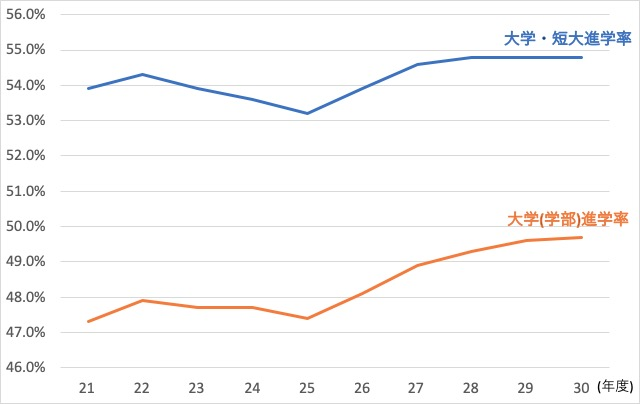
\includegraphics[height=8cm]{images/univ_continuance_rate.jpg}
\caption{過去10年間の大学進学率推移}
\label{fig:univ_continuance_rate}
\end{figure}

一方大学の学校数に関して,日本では774校存在している\ref{fig:university_num}.これは2019年4月の入学者を募集した大学の数である.
それぞれの内訳としては,国立大学が82大学,公立大学が91大学,私立大学が592大学であり,私立大学が全体の約8割を占めている.
このデータのうち,2019年度新設大学は13大学で,内訳は公立大学1校,私立大学10校,専門職大学2校に上る.
また新設学部は国立,私立専門職大学合わせて61学部,新設学科は計118学科となっている.

志願者数の観点から,大学に関する志願者数の推移を日本私立大学振興・共済事業団の資料\cite{shigan}からまとめた.
\begin{figure}[H]
\centering
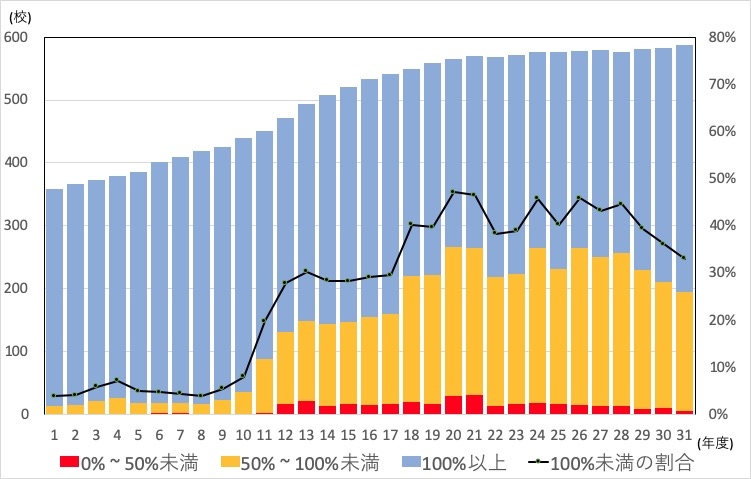
\includegraphics[height=8cm]{images/shigansya.jpg}
\caption{平成元年〜31年の私立大学志願者数の推移}
\label{fig:shigan}
\end{figure}
大学数は増加傾向にあったものの,ここ10年間はほぼ横ばいである.
志願者数が募集人数を下回った大学の比率は近年減少傾向にある.これは2018年から大学に対して入学者の超過率を厳格に制限\cite{hojokin1}したためであると考えられる.
入学者の超過率が厳格に制限されたため,入学者数が絞られる形になり,その分の学生が他の大学に流れた結果定員割れの大学数が減ったと考えられる.
更に平成31年からは入学定員充足率が 0.9 〜 1.0 倍の場合に入学定員充足率に応じて補助金が増額される.\cite{hojokin2}
そのため今後,有名大学の定員は減少傾向になると予想される.
しかしそれでは志願者の一部が第一志望の学校から第二志望の学校になっただけであり,本質的な解決策としては限界がある.

ここで問題として,大学を選ぶ際の基準が画一化しているため,特定の大学に志願者が集中することとなっていると考えた.
大学進学者数は増加傾向にあり,大学数も増加傾向にある.その中で志願者数が偏る原因は,大学選びの基準が画一化していることが原因の一つである.


\section{研究目的}
本研究の目的は,大学に関する記事から各大学の特徴をベクトルで表現し,潜在的な関係性を可視化することを目的とする.
対象とするのは大学受験を控えた高校生で,特定の大学から様々な要素を通して大学間の関係性を可視化することで大学を選ぶ際の基準として機能するか考察する.

\section{関連研究}
類似研究(同じような研究)とは,どこが違うのか(ターゲット,手法,想定結果など)を述べる必要がある.
また,参考にする先行研究(他組織の研究でも良い)とどのような関連性があるのかを述べる.

場合によっては,関連研究が研究目的より先に書いてあった方が「ながれ」が良い場合もある.
また,関連研究を背景の中に入れてしまった方が良いケースもある.
これらについては,文章を書きながら,判断するしかない.

\section{論文構成}
2章では本研究で使用した詳細な技術について説明する.
3章では変研究で提案するシステムの説明と実際に構築したシステムの使用方法を解説する.
4章ではシステムの有効性を検証した結果についてまとめる.
最後に5章で有効性の考察を考察し,本研究のまとめと今後の課題について述べる.